\documentclass{article}
\usepackage{amsmath}
\usepackage{tikz}

\begin{document}

The tuple $(t, s)$ in the orthogonal setting\\
$(t \in \mathbb{S}^{n-1}, s \in \mathbb{S}^{n-2}, t \perp s)$

\begin{center}
    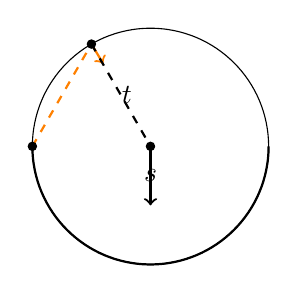
\begin{tikzpicture}[scale=1.5]
        % Draw the sphere
        \draw (0,0) circle (1);
        
        % Draw the great circle
        \draw[thick] (-1,0) arc (180:360:1);
        
        % Draw the tangent vector t
        \draw[orange, dashed, thick] (-1,0) -- (-0.5,0.866);
        \draw[orange, thick, ->] (-0.5,0.866) -- (-0.4,0.7);
        
        % Draw the normal vector s
        \draw[dashed, thick] (-0.5,0.866) -- (0,0);
        \draw[thick, ->] (0,0) -- (0,-0.5);
        
        % Mark points
        \filldraw[black] (-1,0) circle (1pt);
        \filldraw[black] (-0.5,0.866) circle (1pt);
        \filldraw[black] (0,0) circle (1pt);
        
        % Labels
        \node at (-0.2,0.433) {$t$};
        \node at (0,-0.25) {$s$};
    \end{tikzpicture}
\end{center}

\end{document}